\documentclass[11pt]{beamer}
\usepackage{listings} % Include the listings-package
\usepackage[T1]{fontenc}
\usepackage[utf8]{inputenc}
\usepackage[english]{babel}
\usepackage{amsmath}
\usepackage{amssymb, amsfonts, latexsym, cancel}
\usepackage{float}
\usepackage{graphicx}
\usepackage{epstopdf}
\usepackage{subfigure}
\usepackage{hyperref}
%\usepackage{authblk}
\usepackage{blindtext}
\usepackage{booktabs} % Allows the use of \toprule, 
\usepackage{filecontents}
\usepackage{courier} %% Sets font for listing as Courier.
\usepackage{listings}
%\usepackage{listings, xcolor}
\lstset{
tabsize = 2, %% set tab space width
showstringspaces = false, %% prevent space marking in strings, string is defined as the text that is generally printed directly to the console
numbers = left, %% display line numbers on the left
commentstyle = \color{green}, %% set comment color
keywordstyle = \color{blue}, %% set keyword color
stringstyle = \color{red}, %% set string color
rulecolor = \color{black}, %% set frame color to avoid being affected by text color
basicstyle = \small \ttfamily , %% set listing font and size
breaklines = true, %% enable line breaking
numberstyle = \tiny,
}
\usepackage{caption}
\DeclareCaptionFont{white}{\color{white}}
\DeclareCaptionFormat{listing}{\colorbox{gray}{\parbox{\textwidth}{#1#2#3}}}
\captionsetup[lstlisting]{format=listing,labelfont=white,textfont=white}
\definecolor{urlColor}{rgb}{0.06, 0.3, 0.57}
\definecolor{linkColor}{rgb}{0.57, 0.0, 0.04}
\definecolor{fileColor}{rgb}{0.0, 0.26, 0.26}
\hypersetup{
    colorlinks=true,
    linkcolor=linkColor,
    filecolor=fileColor,      
    urlcolor=urlColor,
}
\urlstyle{same}
\setbeamercovered{transparent}
%\usetheme{Boadilla}
\usetheme{CambridgeUS}
%\usetheme{Berkeley}
%\usetheme{Warsaw}
%\usetheme{Madrid}

\title[Introduction]{\bf\Huge Programming introduction}
\subtitle{Fundamentals to programming I}

\author[rescobedoq]
{
	Richart Smith Escobedo Quispe \inst{1}
}
\institute[UNSA]
{
\inst{1}% 
System Engineering School\\
System Engineering and Informatic Department\\
Production and Services Faculty\\
San Agustin National University of Arequipa
}

\date[2020-04-01]{\scriptsize{2020-04-01}}
%\logo{
\includegraphics[width=3.0cm]{img/logo_unsa.jpg}}
\titlegraphic{
\includegraphics[width=3.0cm]{img/logo_unsa.jpg}}

\begin{document}

\begin{frame}
\titlepage
\end{frame}

\begin{frame}
\frametitle{Content}
\tableofcontents
\end{frame}

\section{Von Neumann Architecture}
\begin{frame}
\frametitle{Von Neumann Architecture}
\begin{itemize}
\item John von Neumann (1945).
\item Computer architecture design:
\item Control Unit, Arithmetic and Logic Unit, Registers.
\item Memory Unit.
\item Inputs/Outputs Unit.
\end{itemize}
\end{frame}

\begin{frame}
\frametitle{Von Neumann Architecture}
\begin{center}
{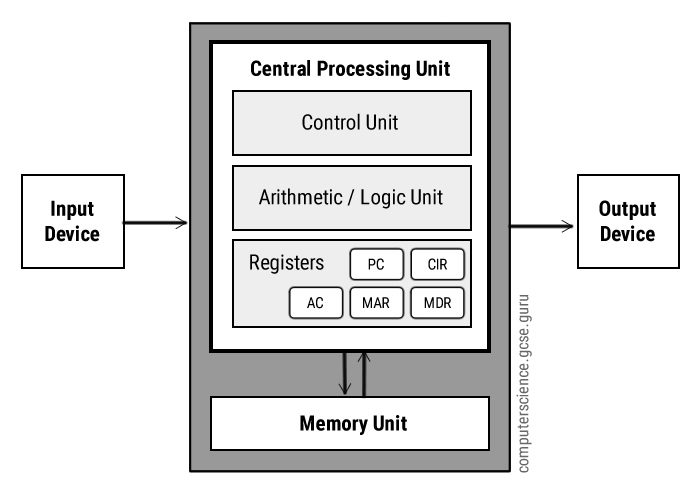
\includegraphics[width=8.0cm]{img/Von-Neumann-Architecture-Diagram.jpg}}
\end{center}
\end{frame}

\section{HelloWorld!}
\begin{frame}
\frametitle{HelloWorld!}
\lstinputlisting[language=Java, label=hello-world, caption=HelloWorld.java]{java/HelloWorld.java}
\end{frame}

\begin{frame}
\frametitle{HelloWorld!}
\begin{center}
{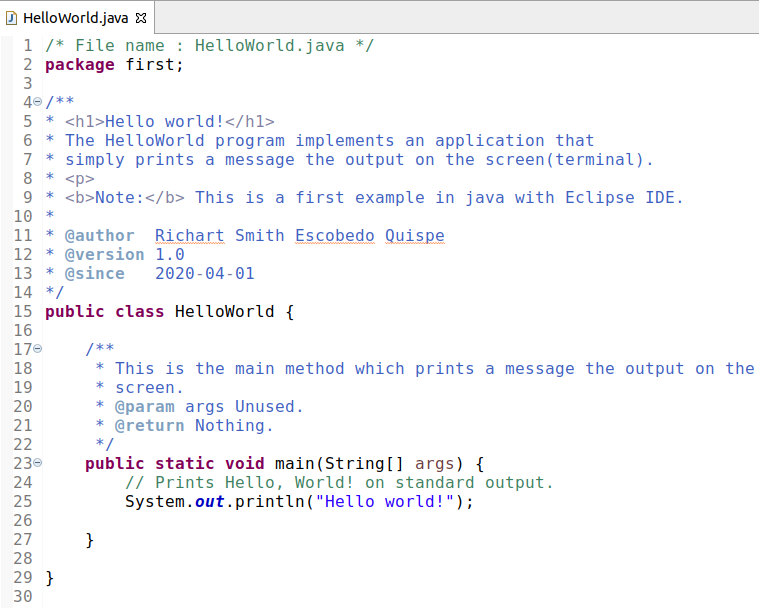
\includegraphics[width=8.0cm]{img/HelloWorld.java.png}}
\end{center}
\end{frame}

\begin{frame}
\frametitle{HelloWorld!}
\begin{center}
{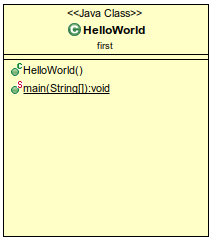
\includegraphics[width=5.0cm]{img/HelloWorld.Java.Class.png}}
\end{center}
\end{frame}



\section{Requirements}
\begin{frame}
\frametitle{Requirements}
\begin{itemize}
\item JDK >=1.8
\item MS Windows, MacOS, GNU/Linux: Oracle
\begin{itemize}
\item jdk-8u261-windows-i586.exe
\item jdk-8u261-windows-x64.exe
\item jdk-8u261-macosx-x64.dmg
\item jdk-8u261-linux-x64.tar.gz (Optional)
\end{itemize}
\item GNU/Linux: Ubuntu 
\end{itemize}
\lstinputlisting[language=Bash, label=openjdk-8, caption=openjdk-8-jdk]{bash/openjdk-8-jdk.sh}
\end{frame}

\section{Create and Run}
\begin{frame}
\frametitle{Create and Run}
\begin{center}
{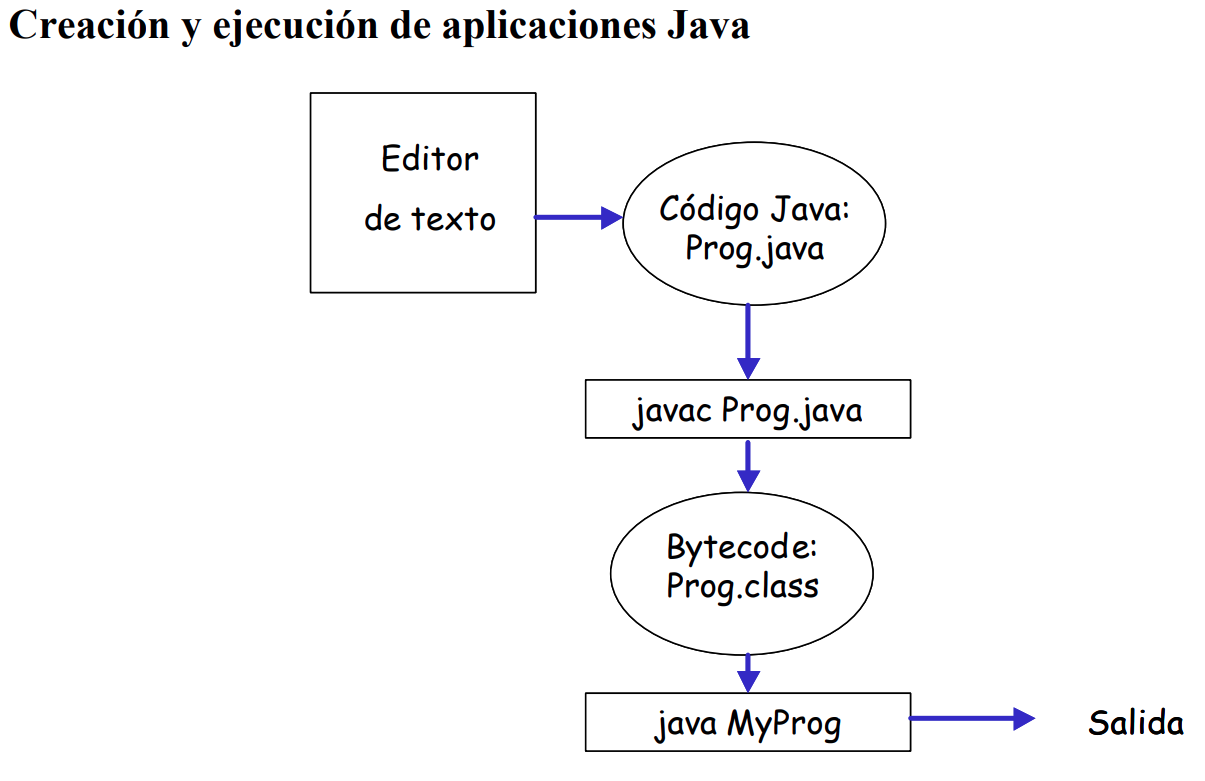
\includegraphics[width=8.0cm]{img/Create_Run_Java.png}}
\end{center}
\end{frame}

\section{Data types}
\begin{frame}
\frametitle{Data types}
\begin{center}
{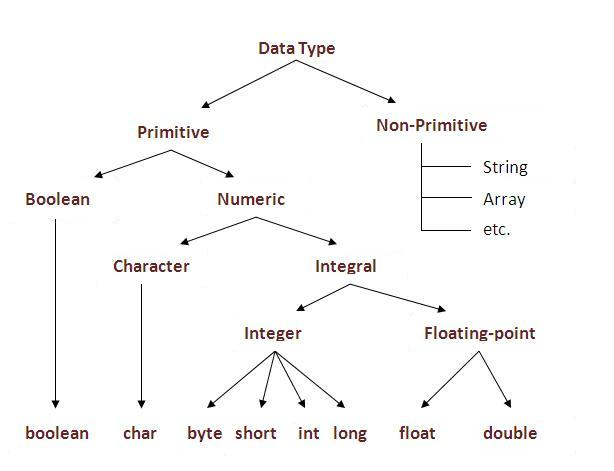
\includegraphics[width=8.0cm]{img/HQoAn.jpg}}
\end{center}
\end{frame}

\begin{frame}
\frametitle{Overflow}
\lstinputlisting[language=Java, label=some-code, caption=Overflow.java]{java/Overflow.java}
\end{frame}

\section{Program: Course.java}
\begin{frame}
\frametitle{Program: Course.java}
\lstinputlisting[language=Java, label=course-java, caption=Course.java]{java/Course.java}
\end{frame}

\section{References}
%References frame
\begin{frame}
\frametitle{References - Web pages}
\begin{itemize}
\item \url{https://elvex.ugr.es/decsai/java/}
\item \url{https://www.oracle.com/java/technologies/javase/javase-jdk8-downloads.html}
\item \url{https://www.eclipse.org/downloads/packages/release/2020-06/r/eclipse-ide-enterprise-java-developers}
\item \url{https://www.objectaid.com/home}
\item \url{https://openjdk.java.net/install/index.html}
\item \url{https://code.visualstudio.com/}
\item \url{https://www.sublimetext.com/}
\item \url{https://vimhelp.org/}
\item \url{https://www.computerscience.gcse.guru/theory/von-neumann-architecture}
\item \url{https://stackoverflow.com/questions/48304498/are-wrappers-of-a-primitive-type-primitives-types-too}
\end{itemize}
\end{frame}

\begin{frame}
\frametitle{References - Books}
\begin{itemize}
\item \href{https://books.google.com.pe/books?id=vJ9QDwAAQBAJ}{Java Fundamentals: Programming Basics for Beginners (2018)}
\item \href{https://books.google.com.pe/books?id=mgFkDwAAQBAJ}{Fundamentals of Java Programming (2018)}
\item \href{https://books.google.com.pe/books?id=urd9DwAAQBAJ}{Java for Absolute Beginners: Learn to Program the Fundamentals the Java 9+ Way (2018)}
\item \href{https://books.google.com.pe/books?id=3RhKDwAAQBAJ}{Java Programming for Beginners: Learn the fundamentals of programming with Java (2017)}
\end{itemize}
\end{frame}

\begin{frame}
\begin{center}
Thanks!...
\
You must review javadoc
\end{center}
\end{frame}

\end{document}
